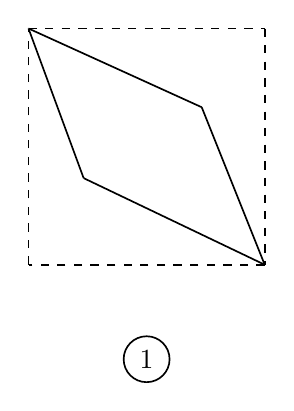
\begin{tikzpicture}[x=1cm,y=1cm,font=\normalsize,
 geometry edge/.style={solid,line width=.6pt},
 geometry mark/.style={solid,line width=.6pt},
 geometry label/.style={font=\normalsize,inner sep=2pt}]
\coordinate (Q1) at (0,3);
\coordinate (Q2) at (3,3);
\coordinate (Q3) at (3,0);
\coordinate (Q4) at (0,0);
\coordinate (P2) at (0.7,1.1);
\coordinate (P3) at (2.2,2.0);
\coordinate (NC) at (1.5,-1.2);
\draw[geometry edge,dashed] (Q1)--(Q2);
\draw[geometry edge,dashed] (Q2)--(Q3);
\draw[geometry edge,dashed] (Q3)--(Q4);
\draw[geometry edge,dashed] (Q4)--(Q1);
\draw[geometry edge] (Q1)--(P3);
\draw[geometry edge] (P3)--(Q3);
\draw[geometry edge] (Q3)--(P2);
\draw[geometry edge] (P2)--(Q1);
\node[draw,circle,inner sep=3pt,line width=.6pt] at (NC) {1};
\end{tikzpicture}